\section{Introduction}
\label{sec:intro}

Language-model agents are increasingly proposed as operators of scientific experimentation:
selecting what to run, interpreting what comes back, and deciding what to run next
\citep{coscientist,chemcrow,szymanski2023autonomous}. The claim attached to this work is
that such agents will accelerate discovery in domains where experiments are the bottleneck.
Whether that claim holds is an empirical question, and answering it requires evaluating
agents under the conditions that make experimentation a bottleneck in the first place.

Existing evaluations do not. In the benchmarks available for automated experimental design,
an experiment is a function call: it returns immediately, costs nothing, and may be repeated
without limit \citep{boxinggym}. Under those conditions the strategy that wins is the one
that queries most, and a poor decision is corrected by making another. Neither property
survives contact with a laboratory. A commercial tomato crop occupies its greenhouse for
seven months and more; a synthesis run consumes reagents and instrument time; a cohort study, once enrolled, cannot be
re-enrolled. In these settings the binding constraint is not the agent's throughput of ideas
but the fact that each idea must be paid for in time and material, and that a design once
committed cannot be revised. An agent optimised against free, instantaneous, repeatable
experiments is being selected on a proxy from which the operative difficulty has been
removed, and we currently have no executable environment in which to find out whether that
selection transfers.

The gap is recognised in the domain literature, which asks for exactly the properties an
idealised environment cannot expose---cost-aware performance, constraint-violation behaviour,
reproducibility (\S\ref{sec:related})---and lacks an environment in which to measure them.

\paragraph{\slowlab.} We introduce an executable benchmark for experimental design under
four conditions that hold at once. Feedback is \textbf{slow}: a cycle is $210$ days, and
the number of trials that run concurrently is capped --- unevenly, because some factors are
set for a whole block of units and others per unit, so replication and coverage compete for
the same physical resource. Observations are \textbf{noisy} enough that one unit does not
settle a question. Experimentation is \textbf{costly} in the objective's own units, since
testing a management regime means growing a crop under it and selling whatever results. And
a submitted design is \textbf{irreversible}: no branch, no checkpoint, no revert. Each
condition alone is familiar. Together they withdraw the recourse every existing benchmark
assumes, because an agent can neither buy precision and coverage from the same units nor
find out which it needed before the season ends.

The conditions define a class rather than a domain --- microbial evolution, bioprocess
scale-up, materials ageing and dose-finding trials satisfy them too, and
Appendix~\ref{app:admit} states what a domain must supply to be admitted. We instantiate
the first in controlled-environment horticulture, where a published mechanistic crop model
\citep{jones1999reduced} coupled to an explicit economic one puts the difficulty outside
our control and every quantity in one currency, net profit per square metre per day
(\S\ref{sec:domain}). The agent's action is a \emph{design}: which factor settings to test,
on how many units, and which physical units those are. Lamps and heating serve a whole
chamber while planting density and the pruning target are set per hydroponic loop, so an
allocation that varies temperature between two loops of one chamber describes an experiment
that cannot be performed. Having committed, the agent sees nothing until the cycle ends;
after two or three cycles it must recommend. Figure~\ref{fig:overview} is the whole loop
on one page.

\begin{figure}[t]
\centering
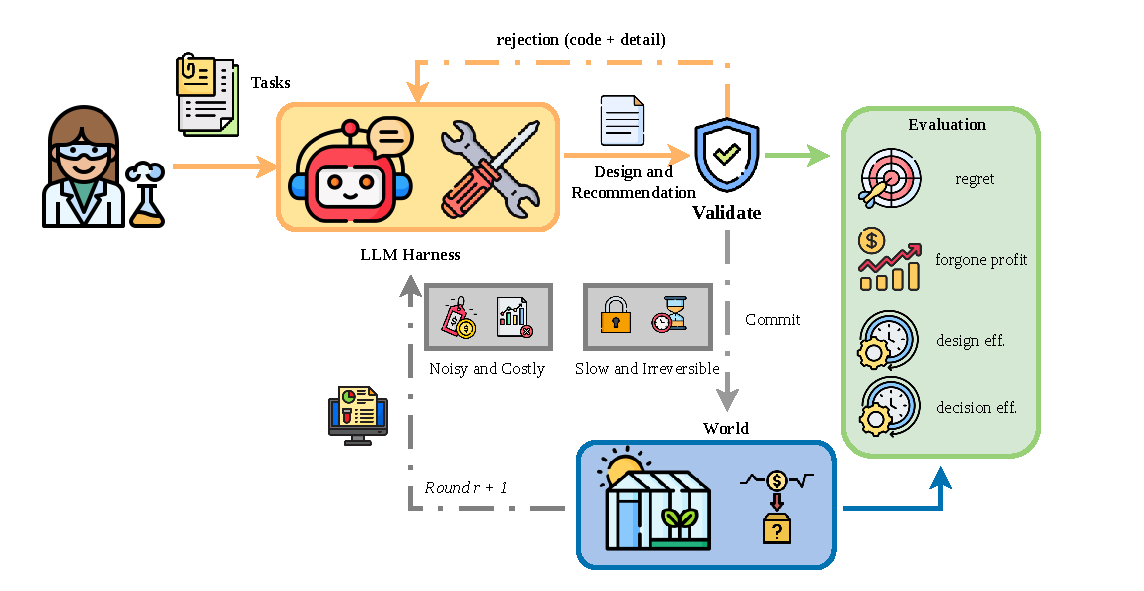
\includegraphics[width=\linewidth]{figures/fig0_overview.pdf}
\caption{\textbf{Overview.} A seed draws a \emph{site}---a parameter vector for the crop
model---from a published between-site spread, unknown to the agent. Each round the harness
serialises the state, the agent returns a complete design and an interim recommendation,
and the design is checked for mechanical feasibility only: a rejection carries a code and a
detail and costs no budget, so the agent may revise without penalty. Committing is the
irreversible step. Committed units are occupied for a full growing cycle---$210$ days, so a
three-round campaign runs for $630$---and the harness returns their values when that cycle
ends. What the agent is denied is not sight of the crop but any action to take on it while
the units are busy. Units are not interchangeable: some factors are set per chamber
and others per loop, so replication and coverage draw on the same physical resource. At the
end the campaign is read three ways: the regret its recommendation realised, the profit its
experiments forwent, and how much of the room its designs closed and its decisions then
used (\S\ref{sec:eval}).}
\label{fig:overview}
\end{figure}

Overall, our work makes the following contributions:
\begin{enumerate}[leftmargin=1.5em,itemsep=3pt,topsep=3pt]
  \item We introduce \slowlab, a \emph{framework for experimental design under slow, noisy,
    costly and irreversible trials}, in which one harness --- protocol, action space,
    feasibility checker, agent interface --- serves a class of domains rather than a single
    one. A domain enters by supplying a published response model, a cost model denominated
    in the objective, and a block structure that makes allocation a decision
    (Appendix~\ref{app:admit}); horticulture is the first, so the optimum is a crop model's
    and not ours to tune.

  \item We introduce a \emph{decision-theoretic measure of design quality}: the regret a
    perfect reasoner would still carry given the design, computed from an instance
    distribution no agent sees. It separates a campaign that could not have answered the
    question from one that could and did not, contains no baseline of ours, and is the
    expected value of sample information --- a batch Knowledge Gradient
    (Appendix~\ref{app:eig}).

  \item We conduct \emph{the first evaluation of language-model agents under these four
    conditions jointly}: five models, four tasks, twenty instances each. We expected
    over-exploration and found the reverse --- most designs use two distinct treatments,
    leaving $99\%$ of six-factor screens unable to separate the effects they were
    commissioned to separate. Supplying a screening tool repairs the designs and makes the
    campaigns end \emph{worse} in sixteen of twenty cells: one intervention, two measures,
    opposite directions.
\end{enumerate}
